%!TEX spellcheck
%!TEX root = ../bachelor_paper.tex
\documentclass[../bachelor_paper.tex]{subfiles}
\graphicspath{{\subfix{images/}}}
\begin{document}

\chapter{Results}
    \label{ch:res}
    
Overall we were able to observe bla bla bla ...
\begin{figure}
    \centering
    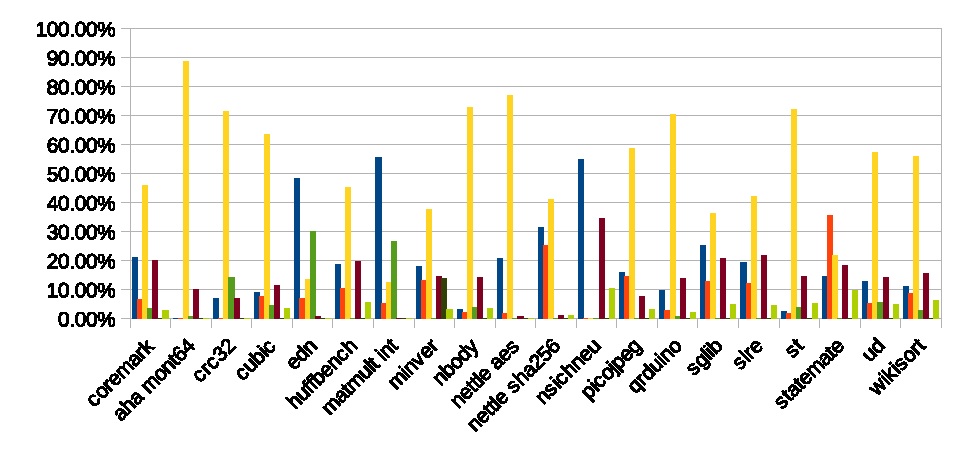
\includegraphics[width=\textwidth]{graph/overall_inst_dist}
    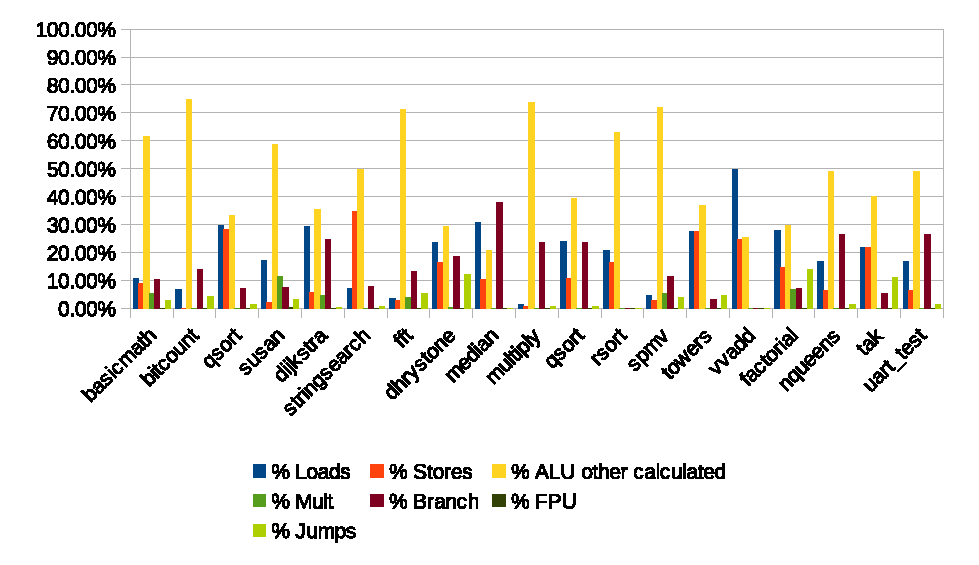
\includegraphics[width=\textwidth]{graph/overall_inst_dist2}
    \caption{Overall instruction distribution of all tested benchmarking workloads}
    \label{fig:res/overall/inst}
\end{figure}

\begin{figure}
    \centering
    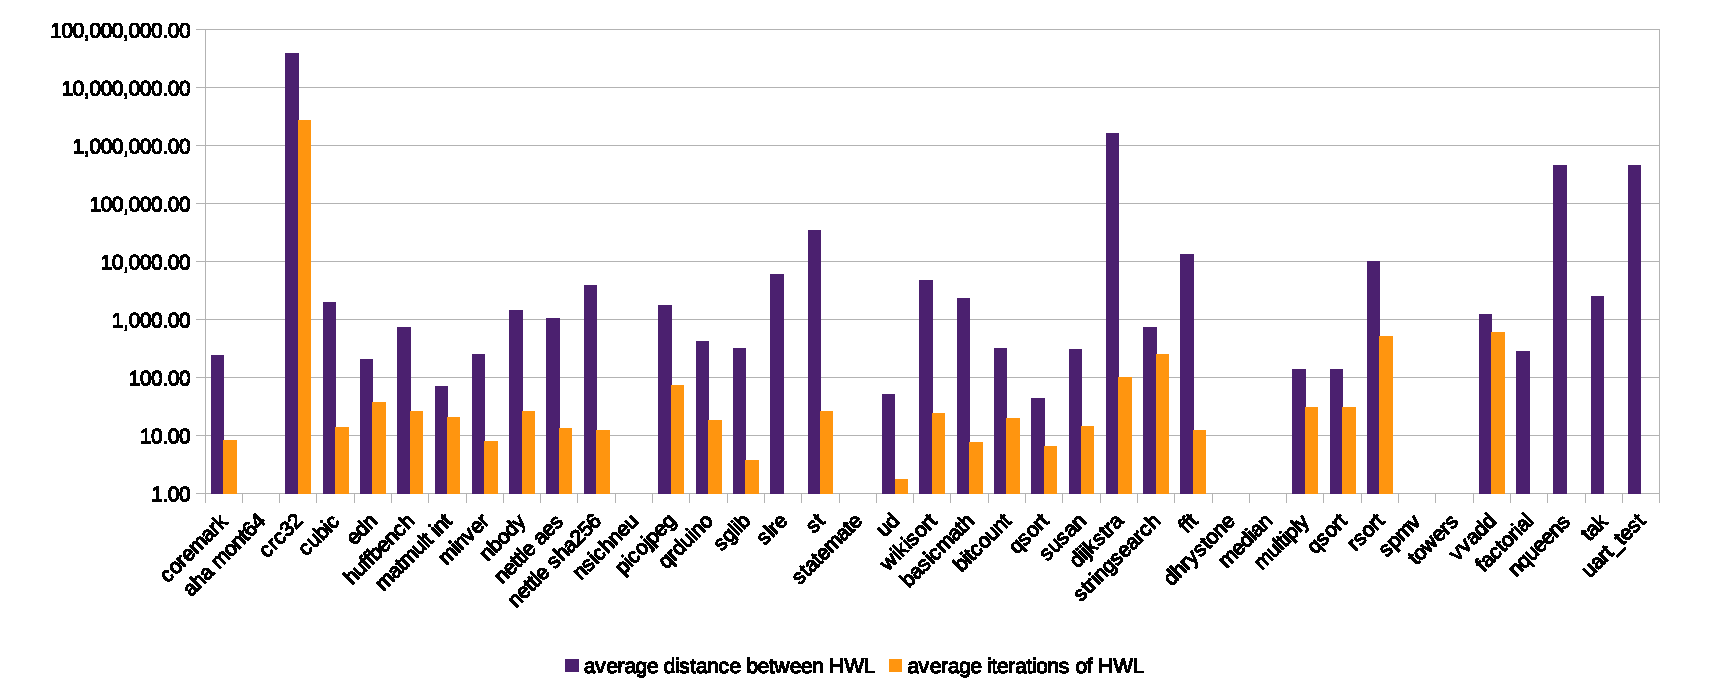
\includegraphics[width=\textwidth]{img/graph/overall_hwl.eps}
    \caption{Overall hardware loop behavior of all tested benchmarking workloads}
    \label{fig:res/overall/hwl}
\end{figure}

\begin{figure}
    \centering
    \includegraphics[width=\textwidth]{img/graph/overall_fetch_waste.eps}
    \caption{Overall load coefficient and cycles wasted per instruction of all tested benchmarking workloads}
    \label{fig:res/overall/fetch_waste}
\end{figure}

\section{Coremark}

\begin{figure}
    \centering
    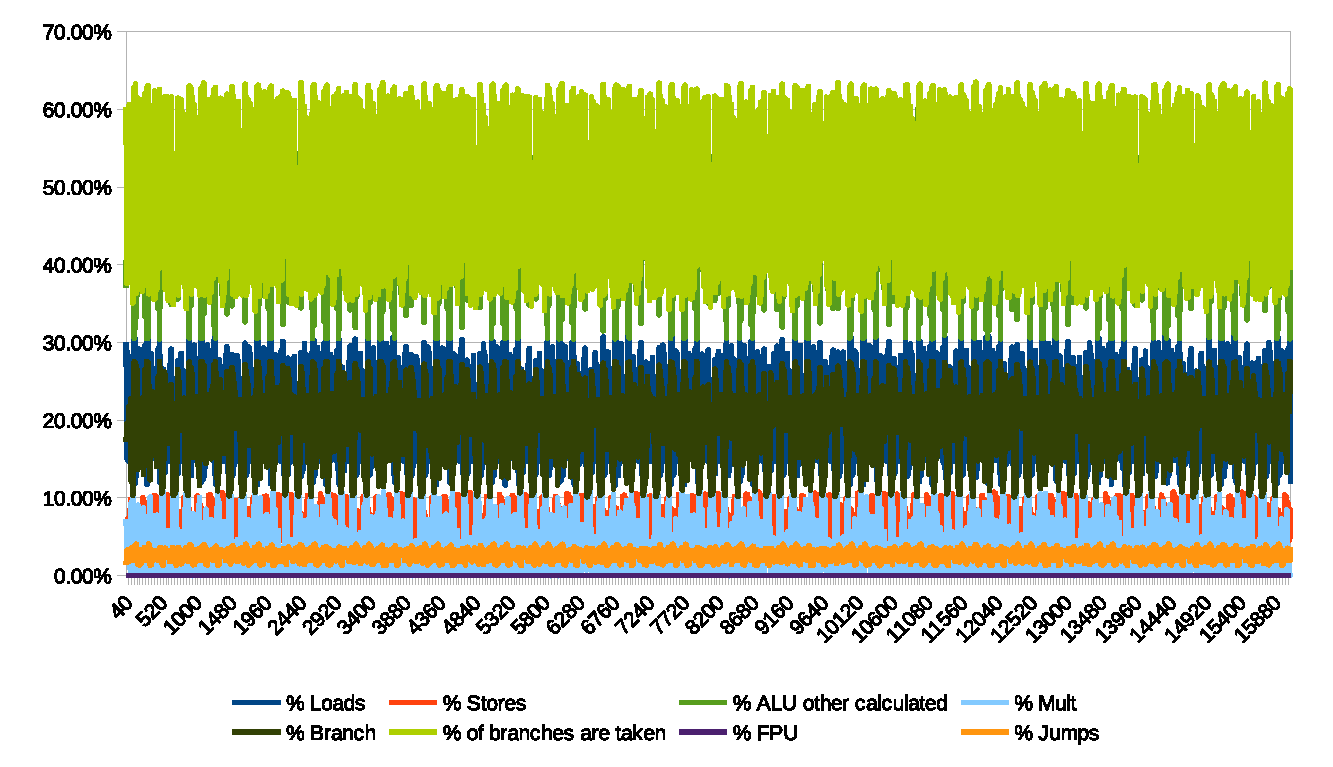
\includegraphics[width=\textwidth]{img/graph/coremark/coremark_inst.eps}
    \caption{Instruction distribution over time of Coremark}
    \label{fig:res/coremark/inst}
\end{figure}

\begin{figure}
    \centering
    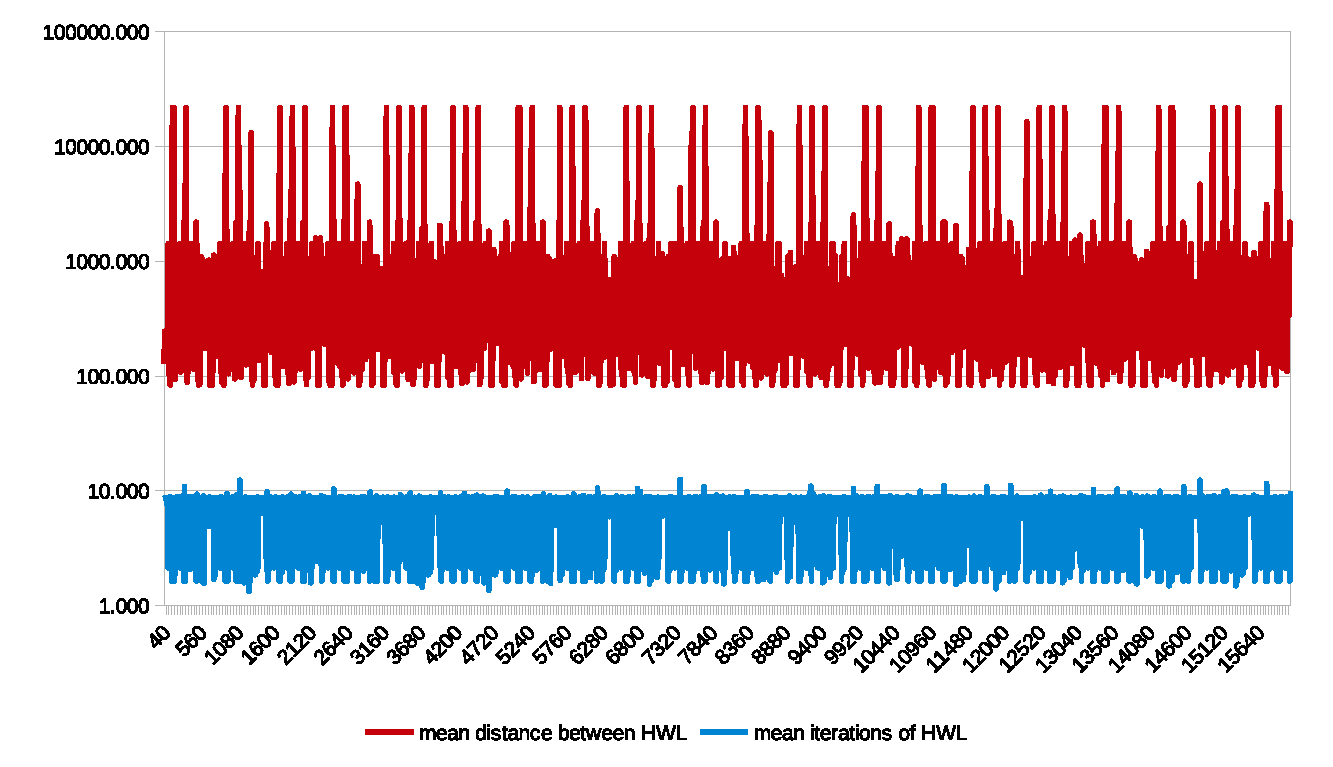
\includegraphics[width=\textwidth]{img/graph/coremark/coremark_hwl.eps}
    \caption{Hardware loop behavior over time of Coremark}
    \label{fig:res/coremark/hwl}
\end{figure}

\begin{figure}
    \centering
    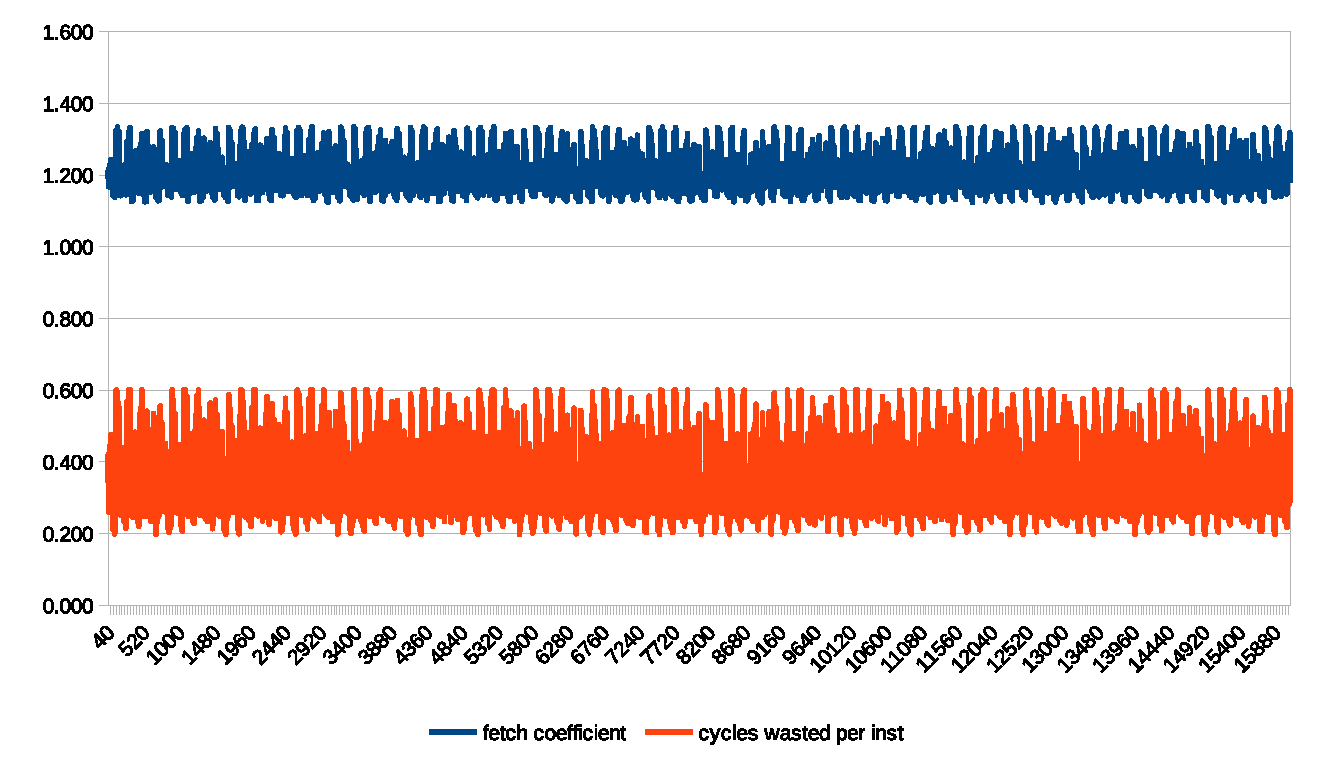
\includegraphics[width=\textwidth]{img/graph/coremark/coremark_fetch_waste.eps}
    \caption{Fetch coefficient and cycles wasted per instruction over time of Coremark}
    \label{fig:res/coremark/fetch_waste}
\end{figure}

% Render bibliograhy and acronyms if rendered standalone
\isstandalone
\bibliographystyle{IEEEtran}
\bibliography{bibliography}
\subfile{abbreviations.tex}
\fi

\end{document} 
